% Supplement to Evans 4.5.3, printed pp. 207--217.
\Needspace{35mm}
\subsection{Geometric optics and stationary phase}\label{sec:4-stationary}
For $u^\varepsilon=a e^{ip/\varepsilon}$ the exact wave-operator identity is
\[
 \begin{aligned}
 &e^{-ip/\varepsilon}(u^\varepsilon_{tt}-\Delta u^\varepsilon)\\
 &\quad=\varepsilon^{-2}a(|Dp|^2-p_t^2)\\
 &\qquad+\frac{i}{\varepsilon}
       \{2p_ta_t-2Dp\cdot Da+a(p_{tt}-\Delta p)\}
       +(a_{tt}-\Delta a).
 \end{aligned}
\]
Matching the first two orders gives the eikonal and amplitude equations
\[
 p_t^2=|Dp|^2,\qquad
 2p_ta_t-2Dp\cdot Da+(p_{tt}-\Delta p)a=0 .
\]
On a smooth nonzero-frequency branch choose $p_t=\pm|Dp|$.
The sign cannot be chosen independently at every point.
For $u_{tt}-\sum a_{ij}(x)u_{x_ix_j}=0$ the first equation becomes
$p_t^2=\sum a_{ij}p_{x_i}p_{x_j}$, with the corresponding amplitude
expression obtained by the same differentiation.
These identities define a candidate expansion.
A theorem about exact solutions needs control of the residual and
the evolution, especially near caustics.
\Needspace{45mm}
\PDEAnnotation{相位误差除以小参数会放大}{即使 $p^\varepsilon-p=o(1)$，也不能直接推出两个指数相近；指数里的差是 $(p^\varepsilon-p)/\varepsilon$。振荡展开需要比普通逐点收敛更精确的误差尺度。}

\begin{lemma}[Nonstationary phase; strengthening source Lemma 1]
If $a\in C_c^\infty$ and $|D\phi|>0$ on its support, then for every
integer $N\geq1$,
$\int e^{i\phi/\varepsilon}a=O(\varepsilon^N)$.
\end{lemma}
\begin{expandedproof}
Near the support let $V=D\phi/|D\phi|^2$.
Then $V\cdot D e^{i\phi/\varepsilon}=(i/\varepsilon)e^{i\phi/\varepsilon}$.
Integration by parts gives
\[
 \int e^{i\phi/\varepsilon}a
 =-\frac{\varepsilon}{i}\int e^{i\phi/\varepsilon}
                                  \operatorname{div}(aV).
\]
Iterate $N$ times; the final smooth compactly supported amplitude
has finite $L^1$ norm independent of $\varepsilon$.
This also proves the source's linear-phase case.
\end{expandedproof}

\begin{lemma}[Quadratic phase; source Lemma 2]
For real symmetric invertible $H$ and $a\in C_c^\infty(\R^d)$,
\[
 \int e^{iz\cdot Hz/(2\varepsilon)}a(z)\,dz
 =(2\pi\varepsilon)^{d/2}
   \frac{e^{i\pi\operatorname{sgn}H/4}}{|\det H|^{1/2}}
      [a(0)+O(\varepsilon)].
 \tag{QP4}
\]
\end{lemma}
\begin{expandedproof}[regularization, branch and error]
For $\operatorname{Re}q>0$,
\[
 \int_{\R} e^{-qs^2+ibs}\,ds=\sqrt{\pi}\,q^{-1/2}e^{-b^2/(4q)} .
\]
Choose the square root with positive real part.
For real positive $q$ this is the Gaussian identity; analytic
continuation in the right half-plane proves it for complex $q$,
since compact subsets admit an integrable Gaussian majorant.
Equivalently the contour argument of Problem 15 proves it directly.

Diagonalize $H$ orthogonally, multiply the phase by
$e^{-\eta|z|^2}$, and apply this identity in each coordinate.
As $\eta\downarrow0$, an eigenvalue $\lambda$ contributes the factor
$|\lambda|^{-1/2}e^{i\pi\operatorname{sgn}\lambda/4}$ after the common
$(2\pi\varepsilon)^{1/2}$ factor.
Insert Fourier inversion for $a$ before this calculation.
Its transform is rapidly decreasing.
The regularized Gaussian integral is uniformly bounded in frequency,
so dominated convergence yields the exact oscillatory identity
\[
 \begin{aligned}
 \int e^{iz\cdot Hz/(2\varepsilon)}a(z)\,dz
 &=C_{\varepsilon,H}(2\pi)^{-d/2}\\
 &\quad\cdot\int \widehat a(\xi)
                e^{-i\varepsilon\xi\cdot H^{-1}\xi/2}\,d\xi ,
 \end{aligned}
\]
where $C_{\varepsilon,H}$ is the prefactor in (QP4).
Since $|e^{ir}-1|\leq|r|$, the bracket differs from $a(0)$ by at most
\[
 C\varepsilon\int |\xi|^2|\widehat a(\xi)|\,d\xi<\infty .
\]
This proves both the constant and the error in (QP4).
\end{expandedproof}

\begin{lemma}[Morse coordinates; source Lemma 3(ii)]
If $D\phi(0)=0$ and $H=D^2\phi(0)$ is invertible, there is a local
smooth diffeomorphism $\Phi$ with $\Phi(0)=0$, $D\Phi(0)=I$, and
$\phi(\Phi(z))=\phi(0)+z\cdot Hz/2$.
\end{lemma}
\begin{expandedproof}[an editorial matrix proof]
Taylor's formula with integral remainder gives
$\phi(x)=\phi(0)+x^TA(x)x/2$, where
$A(x)=2\int_0^1(1-s)D^2\phi(sx)\,ds$ and $A(0)=H$.
On symmetric matrices solve
\[
 H+2S+SH^{-1}S=A(x).
\]
The derivative in $S$ at zero is $2I$, so the implicit function
theorem gives a smooth symmetric $S(x)$ with $S(0)=0$.
Set $B=I+H^{-1}S$; then $B^THB=A$.
The map $z=B(x)x$ has derivative $I$ at zero.
Its local inverse $\Phi$ has the required properties.
This works for indefinite $H$ as well as positive definite $H$.
\end{expandedproof}
For completeness the source's noncritical coordinate lemma is also
elementary. Choose rows $r_1,\ldots,r_{d-1}$ complementary to
$D\phi(0)$, impose $r_j\cdot(y-x)=0$ and
$\phi(y)-\phi(0)=D\phi(0)\cdot x$.
The $y$ Jacobian is invertible; the implicit function theorem
gives $y=\Phi(x)$ and differentiation gives $D\Phi(0)=I$.


\PDEBodyDiagram{4.4}{Near a nondegenerate stationary point the scale is square-root.}
{For phase $x^2$, oscillation is slow near its stationary point at zero and rapid farther away. The highlighted interval has width $2\sqrt{\varepsilon}$. Rescaling $x=\sqrt{\varepsilon}\,z$ explains the leading $\varepsilon^{1/2}$ factor in one dimension; cancellation, not pointwise smallness of the integrand, suppresses the outer region.}
{ch04-stationary-window}

\begin{theorem}[Nondegenerate stationary phase]
Suppose $\phi$ has just finitely many critical points $z_j$ on
$\operatorname{supp}a$, and all $H_j=D^2\phi(z_j)$ are invertible.
Then
\[
 \int e^{i\phi(z)/\varepsilon}a(z)\,dz
 =(2\pi\varepsilon)^{d/2}
 \sum_j\frac{e^{i\phi(z_j)/\varepsilon+i\pi\operatorname{sgn}H_j/4}}
                 {|\det H_j|^{1/2}}
                  [a(z_j)+O(\varepsilon)].
 \tag{SP4}
\]
\end{theorem}
\begin{expandedproof}
Choose a partition of unity separating small neighborhoods of the
critical points from the noncritical compact remainder.
The latter is $O(\varepsilon^N)$ for arbitrary $N$ by the first lemma.
At each critical point change to Morse coordinates.
The transformed amplitude is $a(\Phi(z))|\det D\Phi(z)|$
times its cutoff and equals $a(z_j)$ at the origin.
Apply (QP4) to each localized integral and add them.
Taking $N>d/2+1$ absorbs the noncritical remainder.
\end{expandedproof}
\Needspace{45mm}
\PDEAnnotation{行列式为零时不能继续用驻相公式}{$|\det H|^{-1/2}$ 描述非退化临界点的集中强度。它发散时，表示这一阶近似失效；需研究更高阶相位，不能把发散系数直接当作精确解的无穷大。}

\paragraph{Recovering the rays of Chapter 3.}
For high-frequency displacement $g^\varepsilon(z)=a(z)e^{ip_0(z)/\varepsilon}$
with $|Dp_0|>0$ on $\operatorname{supp}a$ and zero initial velocity,
Fourier representation splits the wave into two equal half-waves.
After frequency rescaling their phases are
\[
 \phi_\pm(x,y,z,t)=(x-z)\cdot y\pm t|y|+p_0(z).
\]
The critical equations are
\[
 y=Dp_0(z),\qquad x=z\mp t\,\frac{Dp_0(z)}{|Dp_0(z)|}.
 \tag{RAY4}
\]
These are exactly the projected HJ rays for $p_t\mp|Dp|=0$.
The joint Hessian at a critical point is
\[
 \begin{pmatrix}
 \displaystyle\pm\frac t{|y|}(I-\widehat y\otimes\widehat y)&-I\\
 -I&D^2p_0(z)
 \end{pmatrix},\qquad \widehat y=y/|y|.
\]
Its determinant equals $(-1)^n$ times the Jacobian determinant
of the ray map in (RAY4), by block elimination.
For small time that map is locally invertible.
The critical value is $p_0(z)$, since
$(x-z)\cdot y\pm t|y|=0$.
Applying (SP4) in $2n$ variables cancels the half-wave prefactor
$(2\pi\varepsilon)^{-n}$ and gives the amplitude
$a(z)/|\det D_zx|^{1/2}$ and the Hessian signature phase.
The two half-waves are then added with weight $1/2$.

The amplitude in $y,z$ is initially not compact in $y$.
To justify this application, first cut frequencies off to a compact
neighborhood of $Dp_0(\operatorname{supp}a)$ disjoint from zero.
Outside that neighborhood $D_z\phi=Dp_0-y$ is nonzero.
Repeated integration by parts in $z$ makes the tail integrable in
$y$, with arbitrarily high powers of $\varepsilon$; for large $y$
each integration also supplies inverse powers of $|y|$.
This reduces to the compactly supported theorem.
The formula is local before caustics or summed over the finitely many
nondegenerate preimages; it asserts no uniform approximation at a caustic.
\par\noindent\begin{minipage}{\linewidth}
\begin{center}
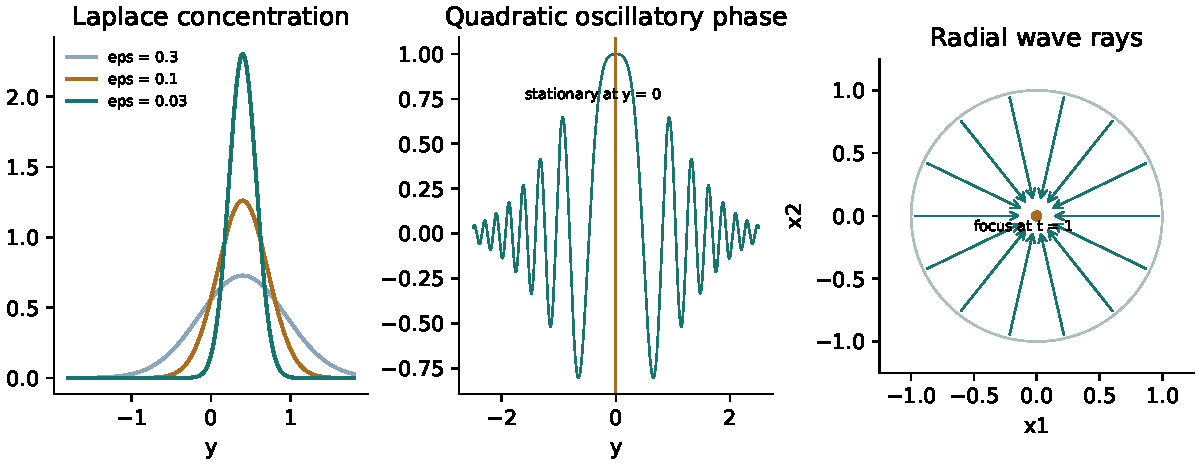
\includegraphics[width=\linewidth]{output/figures/ch04-concentration-rays.pdf}
\end{center}
\noindent\emph{Editorial figure.} Laplace concentration is compared
with oscillatory cancellation; the ray diagram displays a focusing map
whose Jacobian eventually vanishes.
\end{minipage}
